\section{Background} 
\label{sec:bg}
In this section we give a brief overview of DRAM, covering the organization, basic operation, refresh modes, and trends together with projections for the DRAM structure.

DRAM is hierarichally organized as in \reffig{fig:dram_orga}. At the top of the hierarchy are the channels that are connected to one or more ranks, each composed of multiple storage arrays called banks. Each channel has individual address, data, and command buses that makes it possible for the channels to operate cuncurrently. All ranks on one channel can also operate in parallel constrained by the channel bandwith which is shared among the ranks. Further, the banks within the ranks are also able to operate in parallel, but are constrianed by both the shared channel bandwith and resources shared among the banks. 

The DRAM cell array in each bank is structured as in \reffig{fig:dram_orgb}. One cell consists of a transistor and a capacitor, where the transistor is controlled by the wordline wire and connects the capacitor to the bitline wire. The wordline connects a number of cells which forms a row. Each bitline is connected to a sens amplifier and the row of sense amplifier constitutes the row buffer. Data is stored as a charge on the cell capacitor.

\begin{figure*}[t]
    \centering
    \subfigure[DRAM hierarcy]{
        \centering
        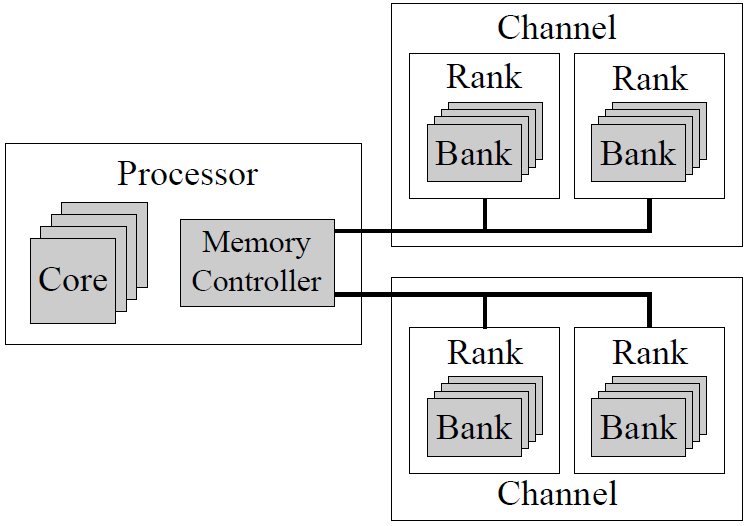
\includegraphics[width=0.4\textwidth]{dram_orga}
		\label{fig:dram_orga}
    }
    \subfigure[DRAM bank structure]{
        \centering
        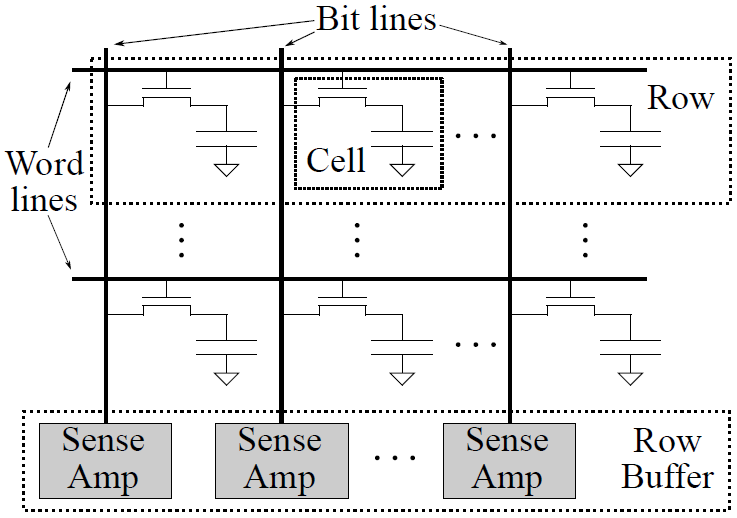
\includegraphics[width=0.4\textwidth]{dram_orgb}
		\label{fig:dram_orgb}
    }
	\caption{DRAM system organization \cite{raidr}.}
	\label{fig:dram_org}
\end{figure*}

To read a row the wordline connected to the rows transistors must first be activated. When the wordline is activated, the transistors connects the capacitors to the bitlines. When the capacitors connects to the bitlines, charge will either flow from or to the capacitors depending on if the capacitors were charged or not, respectively. For this to work, the bitlines has to be precharged to \(V_{DD}\)/2. The sense amplifiers then detect the change of voltage, which makes it possible to interpret the stored data. The charge stored on the capacitors has, as mentioned, left the capacitor and a read operation is thus destructive. To maintain the data the capacitors are recarged by the bitlines, which are driven to either either \(V_{DD}\) or 0 V by the sense amplifiers depending on the former detected voltage change. Finally, if another row on the bank shall be accessed the open row has to be closed, which disconnects the capacitors from the bitlines.

To write to a row the corresponding wordline is first activated. As during a read, the transistors then connects the capacitors to the bitlines and charge will either flow from or to the capacitor. The row buffer are then loaded with the data that are driven to the bitlines by the sense amplifiers, thus storing the information on the capacitors. The row will be closed when another row shall be accessed.

As mentioned, the capacitors leaks charge over time and has to be recharged in order to preserve the data. The refresh is performed by opening a row to let the sense amplifiers amplify the detected voltage change and thus recharge the cells to either \(V_{DD}\) or 0 V. This follows the same procedure as a read operation and thus is the row refreshed when a read is performed. 

The memory controller (MC) normally issues the refresh operation periodically at an interval of 64 ms for each row, an interval that has been constant for the latests DRAM specifications [source]. This interval is halved if the DRAM exeeds the specified working temprature of 85$^{\circ}$C. %The average time between refresh commands are issued by the MC is denoted \(t_{REFI}\) and the time it takes to perform the refresh is denoted \(t_{RFC}\), i.e the time where no normal access requests can be serviced. % Maybe not needed, we shall see.

To refresh one rank, the simplest approach is to refresh all banks in parallel row-by-row at the start of the 64ms interval. This approch is called Burst refresh and has some downsides. The approch blocks normal accesses for a longer period and form a peak of power consumption during the burst time. A better alternative is to distribute the refreshes across the interval, resulting in a lower average latency for the processor and a more stable power consumption.

The implementation of a DRAM refresh cycle can be made in two different ways, to either affect one row or many. The first is called RAS-only refresh (ROR) where refresh cycle refreshes one targeted row. The address for the targeted row has to be put on the bus and it is the MC that makes sure that a row are refreshed within the 64ms interval. The second is called CAS before RAS refresh (CBR). In this scheme the memory module has an internal address counter that displays which row that shall be refreshed. On a refresh cycle, the row stated by the internal address counter is refreshed and the counter is then incremented. The advantage with this method is that the address is never put on the bus, which gives a lower power consumption and less bus usage than ROR. 

When using CBR, all banks in a rank are blocked for normal accesses. All banks are also blocked when ROR is used due to DRAM chip design, however some DRAM chips support per-bank refresh commands that makes it possible to only block the specific bank which is getting refreshed. 

\begin{figure}[t]
    \centering
    \subfigure[DRAM throughput loss]{
        \centering
        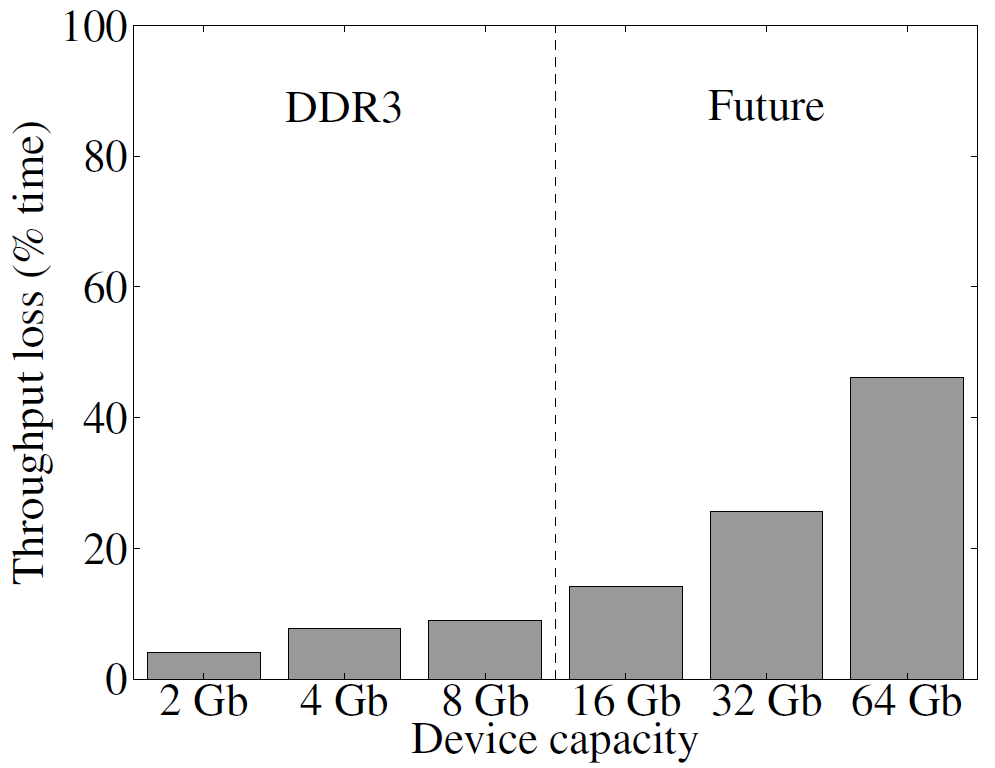
\includegraphics[width=0.33\textwidth]{dram_throughput}
        \label{fig:dram_throughput}
    }
    \subfigure[DRAM power consumption]{
        \centering
        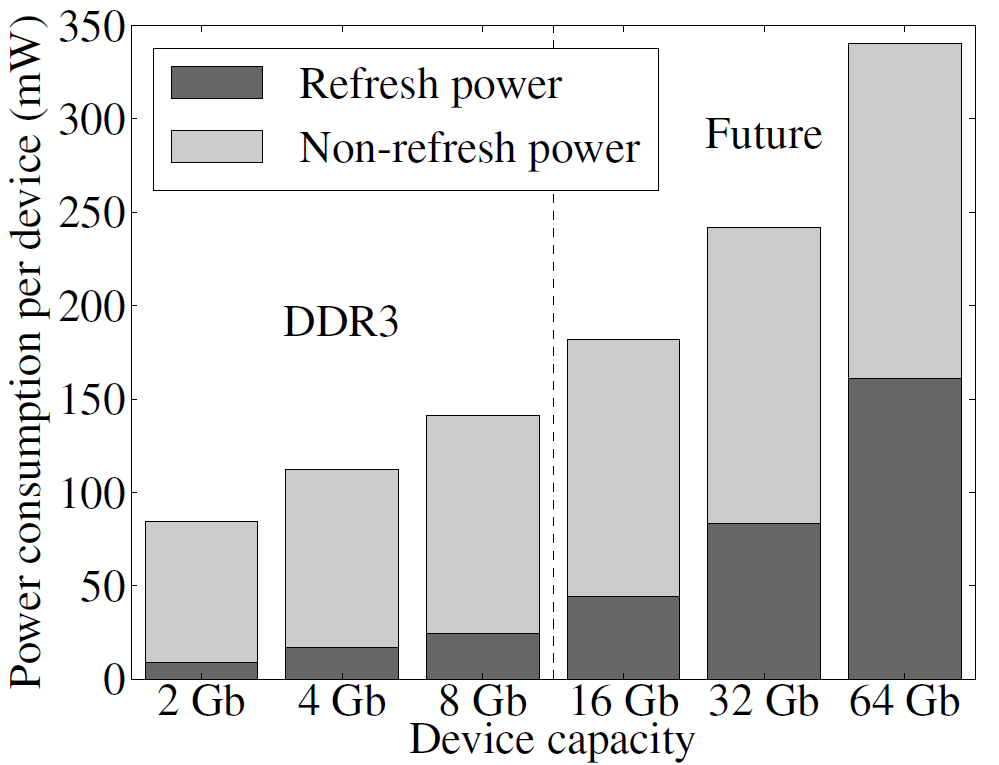
\includegraphics[width=0.33\textwidth]{dram_power}
        \label{fig:dram_power}
    }
    \caption{Projections on DRAM throughput loss and power consumption in extended-temprature operation \cite{raidr}.}
    \label{fig:dram_data_proj}
\end{figure}

The trends of DRAM chips is that they become larger and larger. In practice, this is realized to a high degree by adding additional rows in the banks. The rows could instead - or also - been made longer by adding DRAM cells, but this solution is not favourable as it increases the power consumption per row access. 

As refresh operations are made by row, the refresh operations will increase liniary with the device capacity. In turn, the throughput loss increases exponentially as in \reffig{fig:dram_throughput}. Additional refresh operations gives larger power consumption and the refreshes becomes a growing portion of the total DRAM energy consumption as seen in \reffig{fig:dram_power}. When the device capacity reaches 64 GB the refresh power nearly constitute half of the total consumption, an increase from 15\% if the device capacity is 8 GB. 

\todo[inline]{Drafty stuff below}

In the next years it is projected that ... blablabla [source] so it is important and will be more important in the future to lower the total DRAM power consumption and an relatively easy way to do this is to optimizing the DRAM refresh. Next. we present a bunch of techniques that target DRAM refresh optimization.
